\documentclass{article}
\usepackage{tikz}

\begin{document}

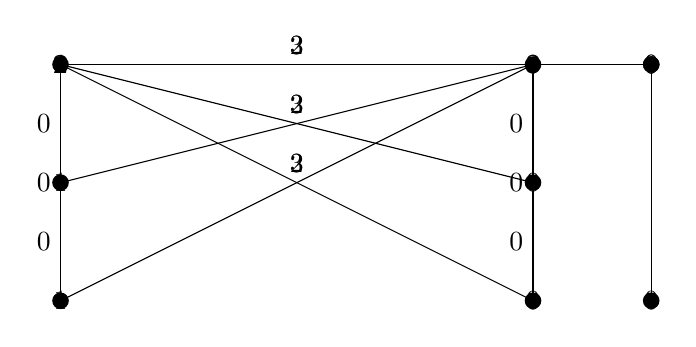
\begin{tikzpicture}[scale=1.5]
    % Define coordinates for the nodes
    \coordinate (A1) at (0,0);
    \coordinate (A2) at (0,1);
    \coordinate (A3) at (0,2);
    \coordinate (B1) at (4,0);
    \coordinate (B2) at (4,1);
    \coordinate (B3) at (4,2);

    % Draw the edges connecting the nodes
    \draw (A1) edge node[left] {0} (A2) 
          (A1) edge node[left] {0} (A3) 
          (A2) edge node[left] {0} (A3)
          (A1) edge node[above] {2} (B3)
          (A2) edge node[above] {2} (B3)
          (A3) edge node[above] {2} (B3)
          (B1) edge node[left] {0} (B2) 
          (B1) edge node[left] {0} (B3) 
          (B2) edge node[left] {0} (B3)
          (B1) edge node[above] {3} (A3)
          (B2) edge node[above] {3} (A3)
          (B3) edge node[above] {3} (A3)
          (B3) -- ++(1,0) coordinate (B3')  -- ++(0,-2) coordinate (B3'')
          (B3') -- ++(-2,0) coordinate (B3''')
          (B3'') -- ++(0,2) coordinate (B3''');
    % Draw the nodes
    \foreach \i in {A1,A2,A3,B1,B2,B3,B3',B3'',B3'''} {
        \fill (\i) circle (2pt);
    }
    % Add labels to the nodes
    \foreach \i/\j in {A1/1,A2/1,A3/1,B1/0,B2/0,B3/0,B3'/0,B3''/0,B3'''/0} {
        \node at (\i) {\j};
    }
    \node at (A3) {\textbf{2}};
    \node at (B3) {\textbf{3}};
\end{tikzpicture}

\end{document}